\subsection{Reinforcement Learning from Human Feedback}
\label{subsec:RLHF}

\subsubsection{Scaling Reinforcement Learning for Generative Reward‑Model Training}
Many recent works \citep{deepseek-genrm,helpsteer3-pref,rmr1} have demonstrated that generative reward models (GenRMs) generalize better than traditional Bradley‑Terry models, reducing the risk of reward hacking during RLHF. In order to train an accurate and robust GenRM, we leverage reinforcement learning at scale. Building on the methodology of \citet{helpsteer3-pref}, we train Qwen3-235B-A22B-Thinking-2507~\citep{yang2025qwen3technicalreport} to become a GenRM with GRPO algorithm.  Given the conversation history, a new user request, and two candidate assistant responses, the GenRM first reasons through the strength and weakness of both responses, then produce an individual helpfulness score for each response as well as a ranking score. For GenRM training, we use 128 prompts per batch, 8 generations per prompt, and do one gradient step on the full batch. We define the reward as

\begin{align}
    \mathbf{R} = -C_1I_{\text{format}} -
    \left| P_{h1} - G_{h1} \right| - \left| P_{h2} - G_{h2} \right| - C_2 \left| P_r - G_r \right|,
\end{align}

where $P_r$, $G_r$ denote the predicted and ground-truth preference rankings; $P_{h1}$, $G_{h1}$, $P_{h2}$, $G_{h2}$ denote the predicted and ground-truth helpfulness scores for responses 1 and 2, respectively;  $I_{format}$ indicates whether the prediction violates the format requirement; $C_1$ and $C_2$ are hyper-parameters controlling the weights. We set $C_1=10$ and $C_2=1$. 

We leverage data from HelpSteer3~\citep{helpsteer3-pref}, a commercially-friendly subset of lmarena-ai/arena-human-preference-140k~\citep{chiang2024chatbot}, and a synthetic safety blend (see details in Appendix~\ref{sec:safety_pref_data}) for model training. In our dataset, individual helpfulness scores range from 1 to 5, where higher means more helpful, while ranking score ranges from 1 to 6, in which 1 denotes that response 1 is far superior to response 2 and 6 denotes that response 2 is far superior to response 1~\citep{helpsteer3-pref}. We augment each sample by switching positions of two responses to prevent positional bias. Figure~\ref{fig:genrm-training} demonstrates that the performance of GenRM on RM-Bench~\citep{rmbench}, JudgeBench~\citep{judgebench}, and our internal validation set steadily improves as training progresses.

\begin{figure}[ht]
    \centering
    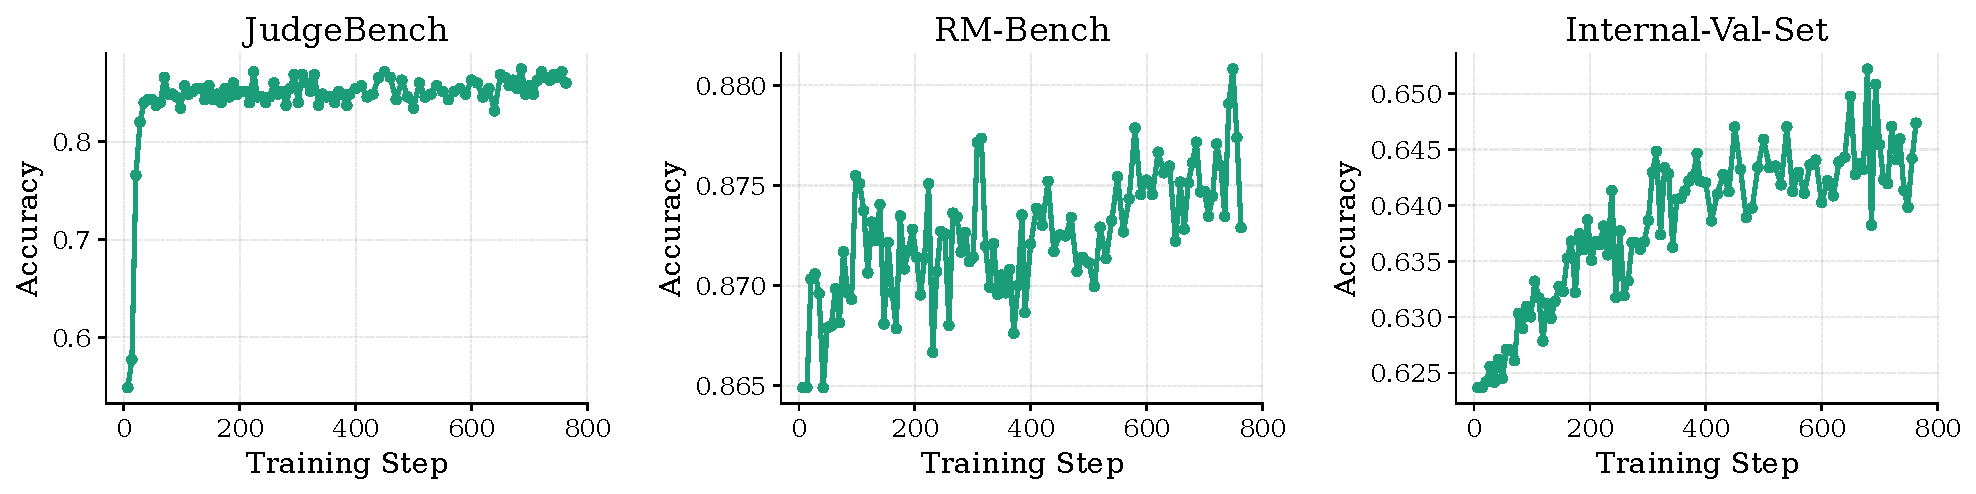
\includegraphics[width=\textwidth]{figures/genrm-training.pdf}
    \caption{GenRM performance improves across benchmarks as we scale up RL training.}
    \label{fig:genrm-training}
\end{figure}
\subsubsection{RLHF with Group Relative Length Control}
With a trained GenRM, we conduct RLHF on the same set of prompts. Same as RLVR, we use a batch of 128 prompts and 16 responses per prompt. Naively comparing all pairs of $N$ responses would require $\binom{N}{2}$ GenRM calls per prompt, which scales quadratically and becomes prohibitively expensive for large $N$. With $N=16$ responses, this would require 120 comparisons per prompt. Instead, we adopt a circular comparison strategy where each response is compared only with its successor: $(r_1, r_2), (r_2, r_3), \ldots, (r_{N-1}, r_N), (r_N, r_1)$, yielding exactly $N$ comparisons. This reduces computational cost from $O(N^2)$ to $O(N)$ while still connecting all responses in a comparison graph. Each response is also judged twice in different positions so as to alleviate positional bias.

For each pairwise comparison $(r_i, r_j)$, the GenRM produces individual helpfulness scores $s_i, s_j \in [1, 5]$ and a ranking score $s_r \in [1, 6]$. In the case where $s_i=s_j$, we further employ a simple tiebreaker mechanism:

\begin{align}
   s_i=s_i+(3.5-s_r), \\
   s_j = s_j + (s_r-3.5).
\end{align}

The base reward $R_i^{(\text{base})}$ for response $r_i$ is then computed by averaging its scores from two matches.

When training with base reward, we find that the length of response can rapidly increase as RLHF training proceeds. This is different from reward hacking, as the increase of length mostly comes from reasoning trace while only final answer is judged by GenRM. It is similar to observations in \citet{deepseekai2025deepseekr1incentivizingreasoningcapability} where model spends more inference time compute to achieve better rewards. However, unlike reasoning heavy tasks like math and coding, prompts in RLHF datasets usually don't require extensive reasoning. In order to reduce redundant thinking, we propose a Group Relative Length Control mechanism during RLHF. Specifically, for each prompt, we generate a group of $N$ candidate responses $\{r_1, r_2, \ldots, r_N\}$. Each response $r_i$ is decomposed into a reasoning component $r_i^{(\text{think})}$ and an answer component $r_i^{(\text{answer})}$, with corresponding lengths $\ell_i^{(\text{think})}$ and $\ell_i^{(\text{answer})}$.



\paragraph{Length-Normalized Reward Adjustment.} We compute a zero-mean, group-relative length bonus that encourages shorter responses within a group. For the reasoning component, we first normalize lengths within the group
\begin{align}
    w_i^{(\text{think})} = 1 - \frac{\ell_i^{(\text{think})} - \ell_{\min}^{(\text{think})}}{\ell_{\max}^{(\text{think})} - \ell_{\min}^{(\text{think})}},
\end{align}

where $\ell_{\min}^{(\text{think})} = \min_j \ell_j^{(\text{think})}$ and $\ell_{\max}^{(\text{think})} = \max_j \ell_j^{(\text{think})}$. To ensure the adjustment is zero-sum across the group (preserving the overall reward scale), we center the weights
\begin{align}
    \tilde{w}_i^{(\text{think})} = w_i^{(\text{think})} - \frac{1}{N}\sum_{j=1}^{N} w_j^{(\text{think})}.
\end{align}

The same procedure is applied to answer lengths to obtain $\tilde{w}_i^{(\text{answer})}$. The final reward for response $r_i$ is then
\begin{align}
    R_i = R_i^{(\text{base})} + \lambda^{(\text{think})} \tilde{w}_i^{(\text{think})} + \lambda^{(\text{answer})} \tilde{w}_i^{(\text{answer})},
\end{align}

where $R_i^{(\text{base})}$ is the base reward from pairwise comparisons and $\lambda^{(\text{think})}, \lambda^{(\text{answer})}$ are  coefficients controlling the strength of the length penalty. We set $\lambda^{(\text{think})}=0.5$, $\lambda^{(\text{answer})}=0.5$.
\paragraph{Quality-Gated Conciseness Bonus.} To further encourage concise responses without sacrificing quality, we introduce optional bonuses for the shortest responses that achieve top-tier quality scores. Let $\tau_p$ denote the $p$-th percentile threshold of scores within the group. For the response $r_k$ with minimum reasoning length:
$$R_k \leftarrow R_k + \beta^{(\text{think})} \cdot \mathbb{1}\left[R_k^{(\text{base})} \geq \tau_p\right]$$
Similarly, for the response $r_m$ with minimum answer length:
$$R_m \leftarrow R_m + \beta^{(\text{answer})} \cdot \mathbb{1}\left[R_m^{(\text{base})} \geq \tau_p\right]$$
where $\beta^{(\text{think})}$ and $\beta^{(\text{answer})}$ are the reasoning and answer conciseness bonuses respectively, and $\mathbb{1}[\cdot]$ is the indicator function. We set $\beta^{(\text{think})}=0.5$, $\beta^{(\text{answer})}=0.5$, and $\tau_p=80$.

This mechanism ensures that (1) length penalties are relative within each prompt group rather than absolute, avoiding bias against inherently complex problems; and (2) conciseness bonuses are only awarded to high-quality responses, preventing the model from learning to produce short but low-quality answers. We observe that the verbosity level reduces 30\% during the training without sacrificing accuracy.

